%%+++++++++++++++++++++++++++++++++++++%%
%%         Final Version  6/14/95      %%
%%+++++++++++++++++++++++++++++++++++++%%
\documentclass[12pt]{article}
\textheight = 8.6in
\textwidth = 6.2in
\topmargin = -.5in
\oddsidemargin = 0.08in
\evensidemargin = 0.08in
%\usepackage{fancyhdr}
%\pagestyle{fancy}
%\rfoot{\thepage}
\setlength{\jot}{10.0 pt}
\setlength{\parskip}{2.0ex}
\setlength{\footskip}{65pt}

\usepackage{graphicx}
\usepackage{subfigure}
\usepackage{placeins}
\usepackage{afterpage}
\usepackage{amsmath}
\usepackage{frcursive}
\usepackage{empheq}
\usepackage[most]{tcolorbox}
\newtcbox{\mymath}[1][]{%
    nobeforeafter, math upper, tcbox raise base,
    enhanced, colframe=white!20!black ,
    colback=blue!30!red!30!white, boxrule=1pt,
    #1}
\usepackage{xcolor}
\definecolor{myblue}{RGB}{0, 0, 180}   %Numbers are integers from 0 to 255, smaller is closer to black


\begin{document}

\begin{flushright} {\color{blue} Chapter 2, Lecture 2} \end{flushright}
\begin{flushleft}

\subsubsection*{\bf Gauss' law}
%\frac{1}{\text{\small\slshape\cursive r}} 
% \frac{1}{4\pi \varepsilon_{0}}
% \text{\small\slshape\cursive r}


It is always possible to find an electrostatic field, $\vec{E}$, by direct integration using Coulomb's law and superposition:

\begin{equation}
\vec{E}=\frac{1}{4\pi \varepsilon_{0}} \int \frac{ \hat{\text{\small\slshape\cursive r}} }{\text{\small\slshape\cursive r}^{2}} dq
\label{eq:intcoul}
\end{equation}

Another method of finding the field is to use Gauss's law, although this is cumbersome unless the charge distribution one of a few convenient symmetries.  These are spherically symmetric charge distributions, infinite lines or cylinders of charge, and infinite planar sheets.  Typical solutions for the fields in these cases are as follows:

\begin{eqnarray*}
 \vec{E}  & = & \frac{ q_{enc} }{ 4 \pi \varepsilon_{0} r^{2}} \, \hat{r} \hspace{.9in} \longrightarrow \hspace{.3in} \mbox{spherical} \\
\vec{E}  & = & \frac{ \lambda_{enc} }{ 2 \pi \varepsilon_{0} s} \, \hat{s} \hspace{.95in} \longrightarrow \hspace{.3in} \mbox{$\infty$ cylinder or line} \\
 \vec{E}  & = & \frac{ \sigma}{ 2 \varepsilon_{0} } \, \hat{n} \hspace{1.1in} \longrightarrow \hspace{.3in} \mbox{$\infty$ sheet} \\
\end{eqnarray*}

Gauss' law is a seemingly magical incantation.  How is it that calculating the flux through a surface of {\it any size} or {\it any shape} surrounding a certain charge gives the same result?  Why do we have so much flexibility in choosing a Gaussian surface?

\subsubsection*{\bf Size doesn't matter (Its what's inside that counts)}

Let's check this out by considering spherical surfaces of different sizes (radii) centered on the same point charge $q$ located at the origin.  Gauss' law says,

\begin{equation}
\oint_{S} \vec{E} \cdot d\vec{a} = \frac{q_{enc}}{\varepsilon_{0}}
\label{eq:gauss}
\end{equation}

We want to show the the flux (LHS of Eq.~\ref{eq:gauss}) is independent of the radius chosen for the Gaussian surface. By Coulomb's law, the electric field on the surface of a sphere of radius $r_{1}$ is given by,

\[
\vec{E}_{1} = \frac{ q }{ 4 \pi \varepsilon_{0} r_{1}^{2} } \, \hat{r}
\]

Substituting $\vec{E}_{1}$ into the flux integral on the left of Eq.~\ref{eq:gauss},

\[
\oint_{S1} \vec{E}_{1} \cdot d\vec{a} = E_{1} \oint_{S1} da = E_{1}(4\pi r_{1}^{2})=\left( \frac{1}{4\pi \varepsilon_{0}}\right) \left( \frac{ q }{r_{1}^{2} } \right)(4\pi r_{1}^{2}) = \frac{q_{enc}}{\varepsilon_{0}}
\]

The result is {\it independent} of the size of the sphere, because although the surface area goes up by a factor of $r^{2}$, the field drops as $\frac{1}{r^{2}}$, and so these scalings cancel.

\subsubsection*{\bf Shape doesn't matter}

OK, but what if the {\it shape} of the Gaussian surface is changed?  We'll take a page out of Feynman's book  (see Feynman lectures), and check it out by comparing the flux due to charge $q$ through a nice spherical shell, to the flux from that same charge through something that looks more like crumpled tin foil.   (See Fig.~\ref{fig:crush})
.
\begin{figure}[h]
\centering
\includegraphics*[trim=0cm 0cm 1cm 0cm, clip=true, width=0.5\columnwidth]{crunch_sphere.png}
\caption{The left sketch shows a point charge surrounded by a spherical shell.  The right sketch shows the same  point charge surrounded by - something else.}
\label{fig:crush}
\end{figure}

Begin by considering one piece of the surface, for example the little patches shown in Fig.~\ref{fig:crush}.  Magnifications of these are shown in Fig.~\ref{fig:sections}.  The left side of Fig.~\ref{fig:sections} shows a patch of the spherical surface defined by two arcs $l$ and $w$.  The right side of Fig.~\ref{fig:sections} shows a patch of the crumpled surface.  One of the arcs ($w$) is chosen to be the same as for the spherical patch, but since the surface is distorted, having an outward tilt in this case, the other side of the patch ($l^{`}$) will not be the same.  Also, whereas the unit normal vector $\hat{n}$ is in the $\hat{r}$ direction for the spherical surface, this is no longer the case of the tilted surface.  There is an angle $\theta$ between $\hat{n}$ and $\hat{r}$ because of the tilt.  If the patch is small enough with respect to the overall size of the surface, the curvature of $w$, $l$, and $l^{`}$ can be neglected, as shown in Fig.~\ref{fig:tilted}.

\begin{figure}[h]
\centering
\includegraphics*[trim=1cm 0cm 0cm 0cm, clip=true, width=0.6\columnwidth]{Gauss_shape1.png}
\caption{\small Magnification of the sections picked out in Fig.~\ref{fig:crush}.  The left sketch shows a patch of a  spherical surface surrounding the point charge.  The right sketch shows a patch of an irregular surface surrounding the point charge. }
\label{fig:sections}
\end{figure}

The flux through the spherical patch is given by,
\[
\Phi_{sph} = \int \vec{E} \cdot d\vec{a} = E \int da = E\Delta a = Elw
\]

The flux through the tilted patch is given by,
\[
\Phi_{tilt} = \int \vec{E} \cdot d\vec{a} =\int E\hat{r} \cdot \hat{n}da = E\cos{(\theta)}\Delta a = E\cos{(\theta)}l^{`}w
\]

\begin{figure}[h]
\centering
\includegraphics*[trim=1cm 0cm 0cm 0cm, clip=true, width=0.6\columnwidth]{Gauss_shape2.png}
\caption{\small A patch on a spherical surface has dimensions $w$ and $l$.  A distorted surface has dimensions $w$ and $l^{`}$ and projects onto a spherical patch that is $w\, \times \, l$.}
\label{fig:tilted}
\end{figure}

Examination of the angles related to the tilted patch in Fig.~\ref{fig:tilted} shows that the angle between $\hat{r}$ and $\hat{n}$ is the same as the angle between $l$ and $l^{`}$.  ($\hat{n} \perp l^{`}$ and $\hat{r} \perp l$)  Then, $\cos{(\theta)}=l/l^{`}$, 

\[
\Phi_{tilt} = E\cos{(\theta)}l^{`}w = E\left( \frac{l}{l^{`}} \right)l^{`}w = Elw = \Phi_{sph}
\]

In the broad view, the reason the shape of the Gaussian surface does not matter is due to the nature of the flux integral.  The dot product of the field with the surface elements picks off only those components of the field perpendicular to the surface.  So, if a Gaussian surface around a spherical distribution of charge is distorted, ultimately only the projection perpendicular to the field matters - and that projection is spherical.

\subsubsection*{\bf Shell theorem}

Getting back to the typcial solutions for various geometries:
\begin{eqnarray}
 \vec{E}  & = & \frac{ q_{enc} }{ 4 \pi \varepsilon_{0} r^{2}} \, \hat{r} \hspace{.9in} \longrightarrow \hspace{.3in} \mbox{spherical} \label{eq:sphere_gauss}\\
\vec{E}  & = & \frac{ \lambda_{enc} }{ 2 \pi \varepsilon_{0} s} \, \hat{s} \hspace{.95in} \longrightarrow \hspace{.3in} \mbox{$\infty$ cylinder or line} \label{eq:cylinder_gauss}\\
 \vec{E}  & = & \frac{ \sigma}{ 2 \varepsilon_{0} } \, \hat{n} \hspace{1.1in} \longrightarrow \hspace{.3in} \mbox{$\infty$ sheet} \label{eq:sheet_gauss}\\
 \nonumber
\end{eqnarray}
the spherical and cylindrical solutions were in terms of $q_{enc}$ and $\lambda_{enc}$, where `enc' is short for `enclosed' meaning only the charge {\it inside} the Gaussian surface contributes to the field at points on that surface.

Another way of expressing this is the `shell theorem'.  Once a spherical Gaussian surface is placed at a specific radius, only the charge lying within the Gaussian surface will contribute to the field at the surface, all outside charge is irrelevant.  Furthermore, if all charge inside the Gaussian surface adds up to total $Q_{total}$, then the field produced by all this charge would be the {\it same} as the field produced by a single point charge of value $Q_{total}$ located at the origin.  In other words, treat all inside charge like a point charge at the center, and ignore all outside charge.

The shell theorem also applies to cylindrical distributions, but in this case all charge inside the Gaussian surface collapses to a line charge along the central axis (not a point).  Again, all outside charge makes no contribution to the field at the location of the Gaussian surface.

\subsubsection*{\bf Example of shell theorem - spherical coordinates}

Suppose a sphere of radius $R$ has a charge density that depends on radial distance from the center, $\rho(r^{`})=A(r^{`})^{2}$, where $A$ is a constant.  What is the electric field at $r=R/2$?  To solve this problem take the following steps:
\begin{enumerate}
\item Put a Gaussian surface where you want to find the field, that is at $r=\frac{R}{2}$.
\item Find the total charge, $q_{enc}$, inside the Gaussian surface, that is at $r\leq \frac{R}{2}$.
\item Apply Eq.~\ref{eq:sphere_gauss}.
\end{enumerate}

The charge inside the Gaussian surface is found by integrating over the charge density.
\begin{equation*}
\begin{aligned}
& \int^{2\pi}_{0} \int^{\pi}_{0}  \int^{\frac{R}{2}}_{0} \rho(r^{`}) d\tau= q_{enc} \\
& \int^{2\pi}_{0} \int^{\pi}_{0}  \int^{\frac{R}{2}}_{0} \rho(r^{`}) \, (r^{`})^{2}\sin{(\theta^{`})}dr^{`}d\theta^{`}d\phi^{`}=q_{enc}\\
& \left[ \int^{2\pi}_{0} d\phi^{`} \int^{\pi}_{0}  \sin{(\theta^{`})}d\theta^{`}\right] \left[ \int^{\frac{R}{2}}_{0} \rho(r^{`})  (r^{`})^{2}dr^{`} \right] =q_{enc} \hspace{.2in} \longrightarrow \hspace{.1in} \mbox{Each integral is independent}  \\
\end{aligned}
\end{equation*}

When a function with only radial dependence is integrated over a volume, the angular portion of the integration is called an {\bf \color{myblue} integration over the solid angle, $\mathbf{\int d\Omega}$}.  This has a value of {\bf \color{myblue} $\mathbf{4\pi}$}, as shown below.
\begin{equation*}
\begin{aligned}
& \int \, d\Omega = \left[ \int^{2\pi}_{0} d\phi^{`} \right] \left[ \int^{\pi}_{0}   \sin{(\theta^{`})}d\theta^{`} \right] \\
& \int \, d\Omega = \left[ \left. \phi^{`} \right\vert_{0}^{2\pi} \, \right] \left[ \left. -\cos{(\theta^{`})} \right\vert_{0}^{\pi} \, \right] \\
& \int \, d\Omega = \left( 2\pi \right) \left[ -( \cos{(\pi)}- \cos{(0)}) \right] = \left( 2\pi \right) \left[ -( -1- 1) \right] = 4\pi\\
\end{aligned}
\end{equation*}

So, getting back to the quest for $q_{enc} \rightarrow $ 
\begin{equation*}
\begin{aligned}
& q_{enc} = 4\pi \int^{\frac{R}{2}}_{0} \rho(r^{`})  (r^{`})^{2}dr^{`}  \\
& q_{enc} = 4\pi  \int^{\frac{R}{2}}_{0} A(r^{`})^{2} (r^{`})^{2}dr^{`}= 4\pi A \int^{\frac{R}{2}}_{0} (r^{`})^{4}dr^{`} \\
& q_{enc}  = 4\pi A \frac{1}{5} \left[ \left. (r^{`})^{5} \, \right\vert_{0}^{\frac{R}{2}} \, \right]  = \frac{\pi A}{40} \, R^{5} 
\end{aligned}
\end{equation*}

Finally, the electric field at $\frac{R}{2}$ is given by,
\begin{eqnarray*}
 \vec{E}_{\frac{R}{2}}  & = & \frac{ q_{enc} }{ 4 \pi \varepsilon_{0} \left( \frac{R}{2} \right)^{2}} \, \hat{r}  \\
 \vec{E}_{\frac{R}{2}}  & = & \frac{ \pi A R^{5} }{ 40 \pi \varepsilon_{0} R^{2}} \, \hat{r}  = \frac{ AR^{3} }{ 40 \varepsilon_{0} } \, \hat{r}\\
\end{eqnarray*}

\subsubsection*{\bf Gauss' law - cylindrical coordinates}

Equation \ref{eq:cylinder_gauss} is the result of applying Gauss' law to an infinite cylindrical distribution of charge.  The simplest distribution of this type is a line charge with linear charge density $\lambda$.  Choose a cylinder for a Gaussian surface because this surface matches the symmetry of the problem.

\begin{figure}[h]
\centering
\includegraphics*[trim=1cm 0cm 0cm 0cm, clip=true, width=0.6\columnwidth]{linecharge.png}
\caption{\small The top sketch shows a line charge with {\it positive} linear charge density $\lambda$ along the central axis of a cylindrical Gaussian surface.  The two bottom sketches show the orientation of the electric field lines with respect to the Gaussian surface; the left sketch shows a side view, and the right sketch shows an end view.}
\label{fig:linecharge}
\end{figure}

The closed surface on the left of the Gauss' law expression becomes three integrals, one for each surface of the cylinder; that is, the two endcaps and the barrel.

\begin{equation*}
\oint_{S} \vec{E} \cdot d\vec{a} = \int_{endcap1} \vec{E} \cdot d\vec{a}+ \int_{endcap2} \vec{E} \cdot d\vec{a} + \int_{barrel} \vec{E} \cdot d\vec{a} =\frac{q_{enc}}{\varepsilon_{0}}
\end{equation*}

If the central axis of the cylinder and the location of the line charge are along the z-axis, then the direction unit  vectors, $\hat{n}$, of the endcaps are in the $\pm \hat{z}$ directions.  The direction of $\hat{n}$ for the barrel is in the $\hat{s}$ direction.  By symmetry, the direction if the electric field, $\vec{E}$ is in the $\hat{s}$ direction, radiating like spokes from the line of (positive) charge.  The contribution to the total surface integral from the endcaps is zero, since $\hat{n} \perp \hat{s}$ for these.  One the other hand, for the barrel, $\hat{n} \, || \, \hat{s}$, so the dot product reduces to a simple product ($\vec{E} \cdot d\vec{a} = Eda$).

\begin{figure}[h]
\centering
\vspace{-.5in}
\subfigure[E field at end of Gaussian surface]
{\label{fig:total}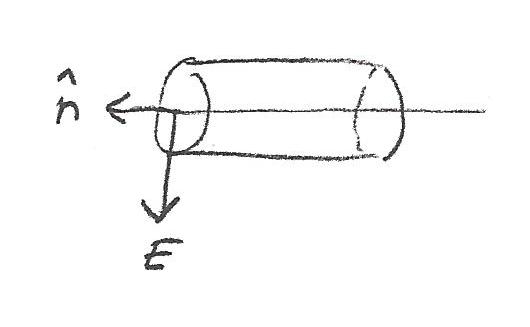
\includegraphics[width=.40\columnwidth]{dir1.png}}
\hspace{.1in}
\subfigure[E field on side of Gaussian surface]
{\label{fig:onesig}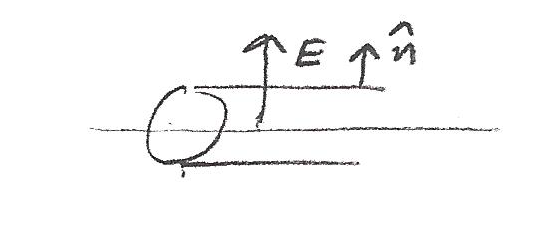
\includegraphics[width=.40\columnwidth]{dir2.png}}
\caption{The left subfigure shows an endcap view of the Gaussian surface with the orientation of the E field and the direction of $\hat{n}$.  The right subfigure is a side view of the Gaussian surface (barrel) showing the orientation of the E field and the direction of $\hat{n}$.}
\label{fig:directions}
\end{figure}

Then, 
\begin{equation*}
\mbox{Flux} = \oint_{S} \vec{E} \cdot d\vec{a} = \int_{barrel} E \, da = E\int_{barrel} da = E (2\pi s)l = \frac{q_{enc}}{\varepsilon_{0}}
\end{equation*}

\begin{figure}[h]
\centering
\includegraphics*[trim=0cm .5cm 0cm 0cm, clip=true, width=0.25\columnwidth]{cylinder.png}
\caption{\small Cartoon showing how to find the area of a cylinder, $A_{cyl}=2\pi \,s \,l$.}
\label{fig:cylinder}
\end{figure}
   
The enclosed charge can be written in terms of the linear charge density and the length $l$ of the cylinder, $q_{enc}=\lambda \, l$.  Gauss' law applied to an infinite wire results in  Eq.~\ref{eq:cylinder_gauss},

\begin{equation*}
\begin{aligned}
&  E (2\pi s)\,l = \frac{ \lambda \, l}{\varepsilon_{0}} \\
&  \vec{E} = \frac{ \lambda }{2\pi \varepsilon_{0} s} \, \hat{s}
\end{aligned}
\end{equation*}

\subsubsection*{\bf Gauss' law - the infinite sheet}

Equation \ref{eq:sheet_gauss} is the result of applying Gauss' law to an infinite planar sheet with surface charge density $\sigma$.  The Gaussian surface of choice is a `pillbox'; this just means a little closed cylinder or rectangular box (this might be handy for storing pills).  The pillbox is placed so that it is intersected by the planar sheet, with the end caps parallel to the sheet (see Fig.~\ref{fig:gaussonsheet}).

\begin{figure}[h]
\centering
\includegraphics*[trim=0cm 0cm 0cm 0cm, clip=true, width=0.3\columnwidth]{pillbox.pdf}
\caption{\small Pillbox Gaussian surface intersecting an infinite sheet of charge that has uniform, positive charge density $\sigma$.}
\label{fig:gaussonsheet}
\end{figure}

Choosing a cylindrical pillbox, once again the flux through the closed surface is found by adding up the flux from the endcaps and the barrel of the cylinder.  Gauss' law for the pillbox is as follows:

\begin{equation*}
\mbox{Flux} = \Phi_{E}=\oint_{S} \vec{E} \cdot d\vec{a} = \int_{endcap1} \vec{E} \cdot d\vec{a}+ \int_{endcap2} \vec{E} \cdot d\vec{a} + \int_{barrel} \vec{E} \cdot d\vec{a} =\frac{q_{enc}}{\varepsilon_{0}} 
\end{equation*}

In this case, symmetry says that the electric field is uniform, and points directly away from the sheet everywhere if $\sigma$ is positive, and directly toward the sheet everywhere if $\sigma$ is negative.  The unit normal vector $\hat{n}$ for the end caps is now parallel to the field (antiparallel if the charge is negative), while $\hat{n}$ for the barrel is perpendicular to the field.  So, only the endcaps contribute to the flux through the pillbox.  In fact, each endcap makes the same contribution; although $\vec{E}$ changes direction on different sides of the sheet, $\hat{n}$ also changes direction.  If the area of the endcaps is $A$, then the flux is,

\begin{equation*}
\Phi_{E}=\oint_{S} \vec{E} \cdot d\vec{a} = 2 \int_{endcap} E\hat{n} \cdot \hat{n} da  = 2E \int_{endcap} da = 2EA = \frac{q_{enc}}{\varepsilon_{0}} 
\end{equation*}

The enclosed charge can be written in terms of the surface charge density and the area $A$ of the endcap, $q_{enc}=\sigma \, A$.  Gauss' law applied to an infinite sheet results in  Eq.~\ref{eq:sheet_gauss},

\begin{equation*}
\begin{aligned}
&  2EA = \frac{ \sigma \, A}{\varepsilon_{0}} \\
&  \vec{E} = \frac{ \sigma }{2\varepsilon_{0}} \, \hat{n}
\end{aligned}
\end{equation*}


\end{flushleft}
\end{document}








